\section{Cơ sở lý thuyết}
\subsection{Các định nghĩa và bổ đề}% co khi xoa 2 cai subsection luon cung duoc}
Phần này giới thiệu một số định nghĩa sẽ được sử dụng trong bài:

\begin{definition}
    Một chuỗi đa giác\footnote{Từ nguyên: polygonal chain} $P = \overline{q_1 q_2 \cdots q_k}$ là chuỗi của các điểm $q_i (i=1, 2, \cdots, k)$ với mỗi cặp $q_i$ và $q_{i+1}$ là một đoạn thẳng và không có hai đoạn thẳng không liên tiếp nào cắt nhau.
\end{definition}

\begin{definition}
    Một đa giác đơn\footnote{Từ nguyên: simple polygon} $n$ đỉnh $P=\left(q_1, q_2, \cdots,q_n\right)$ là một chuỗi đa giác $\overline{q_1 q_2 \cdots q_{n+1}}$ với $q_{n+1} = q_1$. Đường chéo của $P$ là đoạn thẳng $\overline{q_i q_j}, j\ne i + 1$ và không cắt bất kỳ cạnh nào của $P$. Khi đó $P$ được coi như đã \textit{tam giác hóa} nếu phần bên trong nó được chia thành $n-2$ tam giác bởi $n-3$ đường chéo.
\end{definition}

Các đa giác đơn đã tam giác hóa có một tính chất thú vị như sau: Chúng ta có thể xem như đa giác đó là một đồ thị phẳng $G$ trong cùng mặt phẳng. Mỗi tam giác là một miền trong\footnote{Từ nguyên: interior face} của $G$. Từ đó xây dựng đồ thị đối ngẫu $G^D$ của $G$, mỗi mặt của $G$ là một điểm của $G^D$ và mỗi cạnh của $G^D$ được nối từ hai điểm mà mặt của chúng có cạnh chung trong $G$. Khi bỏ đi các điểm thuộc miền ngoài, $G^D$ trở thành một cây (tree) với các đỉnh có bậc tối đa là 3:

\begin{definition}
    Dual tree\footnote{Tạm dịch: cây đối ngẫu} của một đa giác đơn đã tam giác hóa $P$ là một đồ thị $T=(V,E)$ sao cho mỗi nút $V$ tương ứng với một tam giác của $P$ và mỗi cạnh của $E$ được nối bởi hai điểm khác nhau thuộc $V$ nếu tam giác tương ứng của chúng có cạnh chung là một đường chéo của $P$. Đường chéo của $P$ và cạnh tương ứng của $E$ trong $T$ được gọi là \textit{dual}.
\end{definition}


\begin{figure}[h] % h: here, t: top, b: bottom, p: page of floats
  \centering
 \begin{tikzpicture}[scale = 0.65]
%coordinate
    \coordinate (a) at (0,0); \coordinate (b) at (2, 2.5);
    \coordinate (c) at (0,7); \coordinate (d) at (0,13);
    \coordinate (e) at (2, 6); \coordinate (f) at (4.5, 6.25);
    \coordinate (g) at (8, 8.5); \coordinate (h) at (3, 9);
    \coordinate (i) at (5, 12); \coordinate (j) at (12, 10);
    \coordinate (k) at (13,0); \coordinate (l) at (9,0.25);
    \coordinate (m) at (8, 4); \coordinate (n) at (5,0);
    \coordinate (t1) at (0.5, 9); \coordinate (t2) at (1.5, 5);
    \coordinate (t3) at (3, 5.5); \coordinate (t4) at (5, 4.5);
    \coordinate (t5) at (5, 2); \coordinate (t6) at (3, 1);
    \coordinate (t7) at (5, 10); \coordinate (t8) at (8, 10.5);
    \coordinate (t9) at (9,8); \coordinate (t10) at (7, 7);
    \coordinate (t11) at (11, 7); \coordinate (t12) at (10,1);
    \coordinate (s) at (1,5.75); \coordinate (t) at (9.5, 1.5);
%polygon
    \draw[thick] (a) -- (b) -- (c) -- (d) -- (e) -- (f) -- (g) -- (h) -- (i) -- (j) -- (k) -- (l) --(m) -- (n) -- (a);
%diagonal
    \draw[thick, dashed] (c) -- (e); \draw[very thick, dashed] (e) -- (b) node[midway, fill=white] {$d_1$};
    \draw[very thick, dashed] (b) -- (f) node[midway, fill=white] {$d_2$}; \draw[thick, dashed] (b) -- (n);
    \draw[thick, dashed] (b) -- (m); \draw[very thick, dashed] (f) -- (m) node[midway, fill=white] {$d_3$};
    \draw[very thick, dashed] (g) -- (m) node[midway, fill=white] {$d_4$}; \draw[thick, dashed] (g) -- (i);
    \draw[thick, dashed] (g) -- (j); \draw[very thick, dashed] (m) -- (k) node[midway, fill=white] {$d_6$};
    \draw[very thick, dashed] (m) -- (j) node[midway, fill=white] {$d_5$};
%dual tree
    \draw[very thick] (t1) -- (t2) -- (t3) -- (t4) -- (t4) -- (t10) -- (t9) -- (t11) -- (t12);
    \draw[very thick] (t4) -- (t5) -- (t6);
    \draw[very thick] (t9) -- (t8) -- (t7);
%node
    \filldraw[white] (t1) circle (3pt); \draw[thick] (t1) circle (3pt);
    \filldraw[white] (t2) circle (3pt); \draw[thick] (t2) circle (3pt);
    \filldraw[white] (t3) circle (3pt); \draw[thick] (t3) circle (3pt);
    \filldraw[white] (t4) circle (3pt); \draw[thick] (t4) circle (3pt);
    \filldraw[white] (t5) circle (3pt); \draw[thick] (t5) circle (3pt);
    \filldraw[white] (t6) circle (3pt); \draw[thick] (t6) circle (3pt);
    \filldraw[white] (t7) circle (3pt); \draw[thick] (t7) circle (3pt);
    \filldraw[white] (t8) circle (3pt); \draw[thick] (t8) circle (3pt);
    \filldraw[white] (t9) circle (3pt); \draw[thick] (t9) circle (3pt);
    \filldraw[white] (t10) circle (3pt); \draw[thick] (t10) circle (3pt);
    \filldraw[white] (t11) circle (3pt); \draw[thick] (t11) circle (3pt);
    \filldraw[white] (t12) circle (3pt); \draw[thick] (t12) circle (3pt);
    \filldraw[black] (s) circle (3pt) node[above] {$s$};
    \filldraw[black] (t) circle (3pt) node[anchor = north east] {$t$};
%sleeve
    \draw[line width = 2.5pt] (e) -- (f) -- (g) -- (j) -- (k);
    \draw[line width = 2.5pt] (b) -- (m);
    \draw[line width = 2.5pt, dash dot] (e) -- (s) -- (b);
    \draw[line width = 2.5pt, dash dot] (m) -- (t) -- (k);
%arrows
    \draw[thick, latex-] (12.4,6) to [bend right] (14,7) node[above] {Sleeve $P'$};
    \draw[thick, latex-] (8.5, 11) to [bend left] (10,12) node[right] {Đa giác $P$};
    \draw[thick, latex-] (t12) ++(1,-0.5) to [bend right] (13.5,2) node[above] {$\Delta (t)$};
    \draw[thick, latex-] (s) ++(-0.25,0.25) to [bend right] (-0.5,7) node[left] {$\Delta (s)$};
    \draw[thick, latex-] (6.2,6) to [bend left] (4, 7.3) node[above] {Dual tree $G^D$ của $P$};
%buffer
    \filldraw[white] (-1,-1) circle (2pt);
\end{tikzpicture}
  \caption{Đa giác đã tam giác hóa và dual tree của nó.}
  \label{fig:1} % Optional label for referencing
\end{figure} 






Cần chú ý rằng có vô số cách để tam giác hóa một đa giác đơn và một trong những thuật toán sử dụng trong bài này sử dụng thuật toán $O\left(n \log n\right)$ \cite{Triangulate_nlogn}.

Phương pháp của Lee và Preparata dựa trên quan sát sau: Gọi $\Delta (s)$ và $\Delta (t)$ lần lượt là hai tam giác trong $P$ chứa $s, t$ tương ứng. Trong $T$, tồn tại duy nhất đường đi $\pi$ qua các đỉnh của $T$ là các đối ngẫu của $\Delta (s)$ và $\Delta (t)$. Các cạnh trong $\pi$ là đối ngẫu của các đường chéo trong $P$ nên chuỗi các cạnh này tương ứng là chuỗi các đường chéo $d_1, d_2, \cdots,d_p$ theo thứ tự từ $s$ tới $t$. Vì $d_i$ bất kỳ chia $P$ thành hai phần, một chứa $s$ và một chứa $t$ nên đường đi ngắn nhất từ $s$ tới $t$ trong $P$ sẽ phải đi ngang qua mỗi đường chéo $d_1, d_2, \cdots,d_p$ một lần duy nhất. Ta có bổ đề sau (Chứng minh \cite{Lee_paper_proof_lemma_1}):

\begin{lemma}
    Gọi $S$ là tập hợp các đầu mút của các \textit{rào chắn thẳng hàng}. Các đỉnh của đường đi ngắn nhất giữa $s$ và $t$ thuộc $S\cup \left\{s,t\right\}.$
\end{lemma}

Trong trường hợp này, $S$ là tập hợp các đỉnh của $P$. Bồ đề 1 nói ta chỉ cần dựng đường ngắn nhất từ $s$ tới hai đỉnh lần lượt của $d_1, d_2, ...,d_p$ và cuối cùng tới $t$. Hợp của các đường này gọi là cây đường đi ngắn nhất\footnote{Từ nguyên: shortest-path tree} với gốc là $s$. Bởi vì mỗi đường đi từ $s$ đều đi qua một đường chéo một lần duy nhất, ta sẽ đi xây dựng thuật toán tham lam\footnote{Từ nguyên: greedy algorithm}: xét các tam giác lần lượt trên $\pi$, với mỗi tam giác, ta mở rộng cây đường đi ngắn nhất thêm một cạnh và một đỉnh.


\subsection{Thuật toán đề xuất}
Phần này nói về thuật toán tìm được đi ngắn nhất giữa $s$ và $t$ bên trong $P$ thông qua thuật toán mở rộng cây đường đi ngắn nhất từng cạnh một. Bắt đầu với định nghĩa sau:
\begin{definition}
    Một đa giác đã tam giác hóa được gọi là \textit{sleeve}\footnote{Tạm dịch: tay áo} nếu cây đối ngẫu của nó là một chuỗi.
\end{definition}

Với định nghĩa này, ta xây dựng đa giác $P'$ đối ngẫu với $\pi$ sao cho $s, t$ là các đỉnh của đa giác $P'$. Trong phần tiếp theo,  ta sẽ giả sử rằng đa giác $P$ là một sleeve với $n$ đỉnh bao gồm $s$ và  $t$.  

Gọi $v^{(1)}_i$ và $v^{(2)}_i$ lần lượt là hai đầu mút của đường chéo $d_i, 1 \le i \le n -3$,  và gọi $D\left(s, v^{(j)}_i\right)$ là đường đi ngắn nhất từ $s$ tới $v^{(j)}_i, j = 1, 2$ bên trong đa giác $P$. Từ \ref{} $D\left(s, v^{(j)}_i\right)$ là chuỗi bao gồm các đỉnh của  $P$. Gọi $D_i = D\left(s, v^{(1)}_i\right) \cup D\left(s, v^{(2)}_i\right)$, trong $D_i$ tồn tại duy nhất một đỉnh $v$ là đỉnh chung của cả $D\left(s, v^{(1)}_i\right) $ và $ D\left(s, v^{(2)}_i\right)$, và $v$ cách $s$ xa nhất (theo các chuỗi); hay là hai chuỗi $D\left(s, v^{(1)}_i\right) $ và $ D\left(s, v^{(2)}_i\right)$ tách ra tại $v$. 

Giả sử ban đầu không có chuỗi $D$ nào rỗng; ta thấy rằng: $D\left(v, v^{(j)}_i\right) (j=1,2)$ là một chuỗi đa giác lồi vào trong\footnote{Từ nguyên: inward-convex}; nghĩa là phần lồi của nó hướng vào bên trong $P$.  

\begin{proof}
    Xét miền $R_i$  giới hạn bởi $D\left(v, v^{(1)}_i\right), D\left(v, v^{(2)}_i\right)$ và $d_i$  gọi là \textit{phễu}\footnote{Từ nguyên: funnel} nằm trong $P$. Gọi $d_s, d_{s+1}, \cdots, d_{i-1}$ là các đường chéo cắt $D\left(v, v^{(1)}_i\right), D\left(v, v^{(2)}_i\right)$. Dễ thấy tam giác $\left(v, v^{(1)}_s, v^{(2)}_s\right) = R_S$  nằm trong $P$, theo phương pháp quy nạp thì $R_{i-1} \subset P$. Nếu $D\left(v, v^{(1)}_i\right)$ không lồi vào trong, theo bất đẳng thức tam giác, tồn tại một đường đi ngắn hơn từ $v$ tới $v^{(j)}_i$ (xem \ref{fig:2}). Tính chất lồi này chứng minh rằng $D\left(v, v^{(1)}_i\right)$ và $ D\left(v, v^{(2)}_i\right)$ tách ra tại nhiều nhất một đỉnh $v$, nếu chúng tách ra tại một đỉnh $u_1$ khác, nghĩa là chúng phải tái hợp lại tại một đỉnh $u_2$ nào đó; và hai chuỗi phân biệt $u_1, u_2$ mới này phải cùng lồi vào trong.
\end{proof}



\begin{figure}[h] % h: here, t: top, b: bottom, p: page of floats
  \centering
  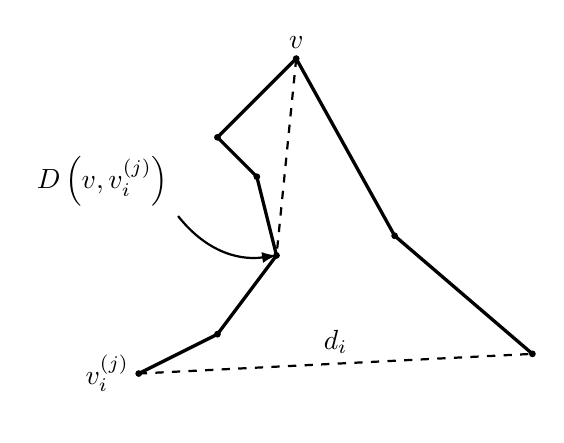
\begin{tikzpicture}[scale = 0.5]
    \coordinate (a) at (0,0);
    \coordinate (b) at (2, 1);
    \coordinate (c) at (3.5, 3);
    \coordinate (d) at (3, 5);
    \coordinate (e) at (2, 6);
    \coordinate (f) at (4, 8);
    \coordinate (g) at (6.5, 3.5);
    \coordinate (h) at (10, 0.5);
    \filldraw[black] (a) circle (2pt) node[left] {$v_i^{(j)}$};
    \filldraw[black] (b) circle (2pt);
    \filldraw[black] (c) circle (2pt);
    \filldraw[black] (d) circle (2pt);
    \filldraw[black] (e) circle (2pt);
    \filldraw[black] (f) circle (2pt) node[above] {$v$};
    \filldraw[black] (g) circle (2pt);
    \filldraw[black] (h) circle (2pt);
    \draw[very thick] (a) -- (b) -- (c) -- (d) -- (e) -- (f) -- (g) -- (h);
    \draw[thick, dashed] (a) -- (h) node[above, midway] {$d_i$};
    \draw[thick, dashed] (f) -- (c);
    \draw[thick] [-latex] (1, 4) to [bend right] (c);
    \draw (1, 4) node[anchor=south east] {$D\left(v,v_i^{(j)}\right)$};
    \draw[white] (-1,-1) circle (1pt);
\end{tikzpicture}
  %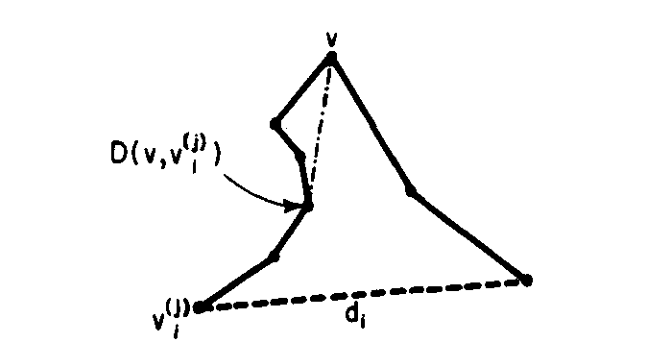
\includegraphics[width=0.7\textwidth]{Images/BTL[image]/lee_fig2.png} % Replace with your image file and path
  \caption{Minh họa về sự lồi vào trong của $D\left(s,v^{(j)}_i\right)$.}
  \label{fig:2} % Optional label for referencing
\end{figure} 





Tổng quát đối với $D_i$, các chuỗi tách ra tại đỉnh $v$ nào đó được gọi là \textit{đỉnh phễu}\footnote{Từ nguyên: cusp} của hai chuỗi lồi vào trong. Chú ý rằng một trong hai chuỗi có thể rỗng nhưng không thể cả hai vì $v^{(1)}_i \ne v^{(2)}_i$. Nếu $D\left(v, v^{(1)}_i\right)$ rỗng thì thì $D\left(v,v^{(2)}_i\right) = d_i$.
\newpage
Thuật toán xây dựng $D_1,D_2,\cdots,D_p$ và cuối cùng $D\left(s,t\right)$. Chi tiết:

\begin{algorithm}
\caption{Xây dựng chuỗi $D_i$}
\begin{algorithmic}
    \STATE \textbf{Ban đầu:} nối $s$ với $v^{(1)}_1$ và $v^{(2)}_1$ để tạo $D_1$.
    \STATE \textbf{Tổng quát:} Để tạo ra $D_{i+1}$ từ $D_i$:
    \STATE Gọi $v$ là đỉnh phễu của $D_i$, tại đỉnh hai chuỗi $\overline{u_a u_{a+1} \cdots u_b}$ và $\overline{u_a u_{a-1} \cdots u_0}$ tách ra, $v = u_a, v^{(1)}_i = u_b, v^{(2)}_i = u_0$. Không mất tính tổng quát: $v^{(1)}_i = v^{(1)}_{i+1}$. Bắt đầu từ $u_0$, gọi $j$ là số nguyên nhỏ nhất mà $\overline{v^{(2)}_{i+1} u_j}$ trở thành \textit{đường hỗ trợ}\footnotemark của đường biên của $R_i$. Xét hai trường hợp:
    \begin{itemize}
        \item [(i)] $j \leq a$. Xóa tất cả cạnh $\overline{u_l u_{l+1}}, 0 \leq l \leq j -1$ và thêm cạnh $\overline{u_j v^{(2)}_{i+1}}$.
        \item [(ii)] $j > a$. Xóa tất cả cạnh $\overline{u_l u_{l+1}}, 0 \leq l \leq j -1$ và thêm cạnh $\overline{u_j v^{(2)}_{i+1}}$; $u_j$ trở thành đỉnh phễu mới của $R_{i+1}$.
    \end{itemize}

    \STATE \textbf{Bước cuối:} Khi xây dựng xong $D_{n-3}$, ta xem như có thêm một đường chéo chứa $t$ (đường chéo $d_{n-2}$) và áp dụng lại bước Tổng quát ở trên.
    \STATE \textbf{Kết quả:} $D\left(s,t\right)$
\end{algorithmic}
\end{algorithm}

\begin{figure}[h] % h: here, t: top, b: bottom, p: page of floats
  \centering
  %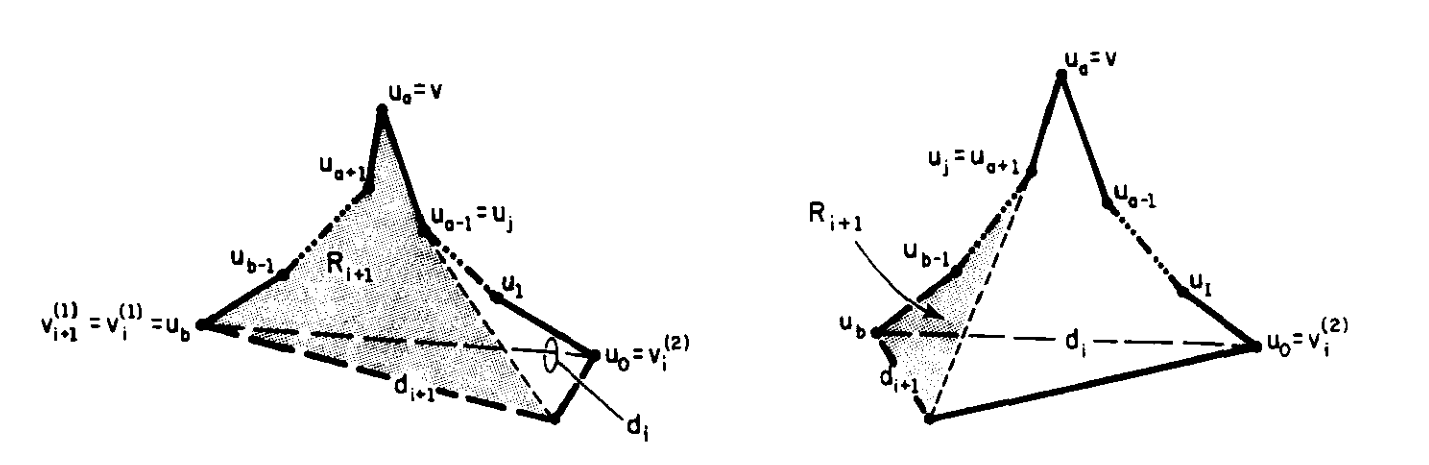
\includegraphics[width=0.95\textwidth]{Images/BTL[image]/lee_fig3.png} % Replace with your image file and path
 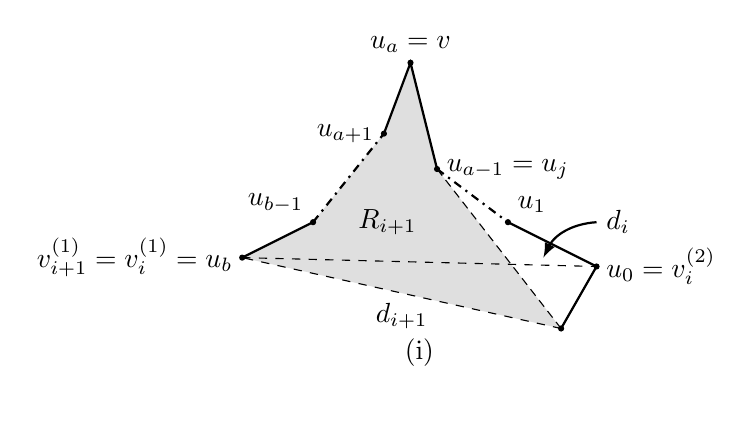
\begin{tikzpicture}[scale = 0.45]
    \coordinate (a) at (0,0);
    \coordinate (b) at (2, 1);
    \coordinate (c) at (4, 3.5);
    \coordinate (d) at (4.75, 5.5);
    \coordinate (e) at (5.5, 2.5);
    \coordinate (f) at (7.5, 1);
    \coordinate (g) at (10, -0.25);
    \coordinate (h) at (9, -2);
    \fill[lightgray, opacity = 0.5] (a) -- (b) -- (c) -- (d) -- (e) -- (h) -- cycle;
    \filldraw[black] (a) circle (2pt) node[left] {$v_{i+1}^{(1)} = v_i^{(1)} = u_b$};
    \filldraw[black] (b) circle (2pt) node[anchor = south east] {$u_{b-1}$};
    \filldraw[black] (c) circle (2pt) node[left] {$u_{a+1}$};
    \filldraw[black] (d) circle (2pt) node[above] {$u_a = v$};
    \filldraw[black] (e) circle (2pt) node[right] {$u_{a-1} = u_j$};
    \filldraw[black] (f) circle (2pt) node[anchor = south west] {$u_1$};
    \filldraw[black] (g) circle (2pt) node[right] {$u_0 = v_i^{(2)}$};
    \filldraw[black] (h) circle (2pt);
    \draw[thick] (a) -- (b);
    \draw[thick, dash dot] (b) -- (c);
    \draw[thick] (c) -- (d) -- (e);
    \draw[thick, dash dot] (e) -- (f);
    \draw[thick] (f) -- (g) -- (h);
    \draw[densely dashed] (e) -- (h);
    \draw[dashed] (h) -- (a) node[midway, below] {$d_{i+1}$};
    \draw[dashed] (a) -- (g);
    \draw (3,1) node[right] {$R_{i+1}$};
    \draw[thick] [latex-] (8.5, 0) to [bend left] (10, 1);
    \draw (10,1) node[right] {$d_i$};
    \draw (5, -2) node[below] {(i)};
    \draw[white] (0,-4) circle (2pt);
\end{tikzpicture}
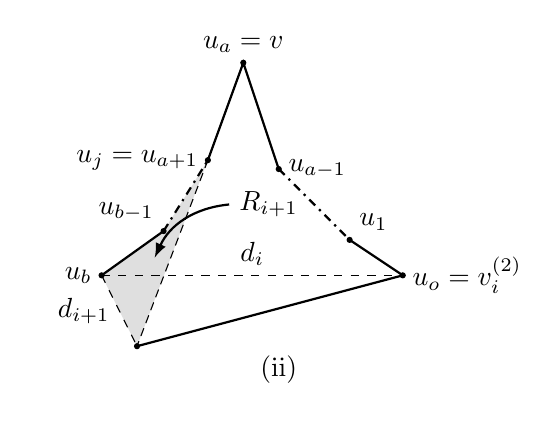
\begin{tikzpicture}[scale = 0.45]
    \coordinate (a) at (0,0);
    \coordinate (b) at (1.75, 1.25);
    \coordinate (c) at (3, 3.25);
    \coordinate (d) at (4, 6);
    \coordinate (e) at (5, 3);
    \coordinate (f) at (7, 1);
    \coordinate (g) at (8.5, 0);
    \coordinate (h) at (1, -2);
    \fill[lightgray, opacity = 0.5] (a) -- (b) -- (c) -- (h) -- cycle;
    \filldraw[black] (a) circle (2pt) node[left] {$u_b$};
    \filldraw[black] (b) circle (2pt) node[anchor = south east] {$u_{b-1}$};
    \filldraw[black] (c) circle (2pt) node[left] {$u_j = u_{a+1}$};
    \filldraw[black] (d) circle (2pt) node[above] {$u_a = v$};
    \filldraw[black] (e) circle (2pt) node[right] {$u_{a-1}$};
    \filldraw[black] (f) circle (2pt) node[anchor = south west] {$u_1$};
    \filldraw[black] (g) circle (2pt) node[right] {$u_o = v_i^{(2)}$};
    \filldraw[black] (h) circle (2pt);
    \draw[thick] (a) -- (b);
    \draw[thick, dash dot] (b) -- (c);
    \draw[thick] (c) -- (d) -- (e);
    \draw[thick, dash dot] (e) -- (f);
    \draw[thick] (f) -- (g) -- (h);
    \draw[dashed] (a) -- (h) node[midway, left] {$d_{i+1}$};
    \draw[dashed] (a) -- (g) node[midway, above] {$d_i$};
    \draw[densely dashed] (c) -- (h);
    \draw[thick, latex-] (1.5, 0.5) to [bend left] (3.6, 2) node[right] {$R_{i+1}$};
    \draw (5, -2) node[below] {(ii)};
    \draw[white] (-2,0) circle (2pt);
    \draw[white] (0,-4) circle (2pt);
\end{tikzpicture}
 
  \caption{Hai trường hợp của bước tổng quát.}
  \label{fig:3} % Optional label for referencing
\end{figure} 



\footnotetext{Từ nguyên: supporting line. \textit{l} là đường hỗ trợ của một đường cong \textit{C} nếu nó có một điểm chung với \textit{C} và \textit{C} nằm toàn bộ ở một phía của \textit{l}}

\hspace{15cm}

Tính đúng đắn của thuật toán dựa trên nhận xét sau: Với mọi $u$ trong tam giác $R_{i+1}$ xác định bởi hai đường chéo $d_i, d_{i+1}$, đường đi ngắn nhất từ $s$ đến $u$ đi qua $v$ là đỉnh phễu của $D_i$. Hiển nhiên đúng với $i = 1, v=s$. Ta đi chứng minh bằng quy nạp như sau:

\begin{proof}
    giả sử đúng tới $1, \cdots, i -1$; xét hai chuỗi $D\left(v, v^{(1)}_i\right), D\left(v, v^{(2)}_i\right)$. Nếu một trong hai chuỗi là rỗng, chuỗi còn lại sẽ bao gồm $d_i$ với $v$ trở thành đỉnh của $d_i$. Trong trường hợp này, đường đi ngắn nhất từ $s$ tới $u$ phải là đoạn ngắn nhất của $D(s,v)$ và đoạn thẳng $\overline{vu}$, và hoàn tất chứng minh. Nếu cả hai chuỗi đều không rỗng, xét cạnh kề với đỉnh $v$ trên bất kỳ chuỗi con nào. Vì $P$ là sleeve, ít nhất một trong số chúng là đường chéo của $P$ (kể cả khi nó không phải đường chéo có được từ thuật toán tam giác hóa $P$). Gọi $\overline{v v'}$ là đường chéo và $\overline{v v^{"}}$ không phải đường chéo. Bởi vì sự lồi vào trong của hai chuỗi, các tia tạo bởi $\overline{v v'}$ và $\overline{v v^{"}}$ cắt $R_{i+1}$ thành ba phần. Điểm $u$ sẽ thuộc một trong ba phần này; cả ba trường hợp đều tương tự nhau. Giả sử đường ngắn nhất từ $s$ tới $u$ là chuỗi $l(s,u)$ không đi qua $v$ mà thay vào đó cắt $\overline{v v^{'}}, \overline{v v^{"}}$ tại $p \neq v, p_1 \neq v$. Theo định nghĩa đường đi ngắn nhất:    
    \[ length\left(l(s,p)\right) + length\left(l(p,p_1)\right) < length\left(D(s,v)\right) + length\left(\overline{v p_1}\right)  \]
    theo bất đẳng thức tam giác: 
    \[ length\left(D(s,v)\right) + length\left(\overline{vp}\right) - length\left(l(s,p)\right) > 0 \]
    Từ đó: 
    \[ length\left(D(s,v)\right) + length\left(\overline{vv'}\right) > length\left(l(s,p)\right) + length\left(\overline{pv'}\right) \]
    Trường hợp này mâu thuẫn với trường hợp đầu là đường ngắn nhất từ $s$ tới $v'$ là qua $v$.
\end{proof}

\newpage

\begin{figure}[h] % h: here, t: top, b: bottom, p: page of floats
  \centering
  %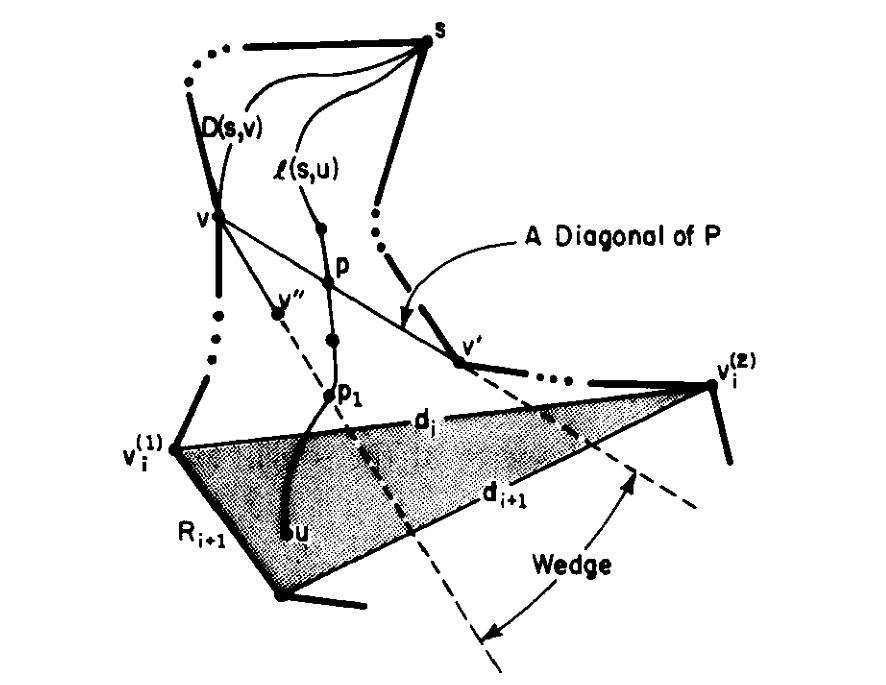
\includegraphics[width=0.65\textwidth]{Images/BTL[image]/lee_fig4.png} % Replace with your image file and path
  \begin{tikzpicture}[scale = 0.8]
  \coordinate (a) at (-1,0);
  \coordinate (b) at (1.25, 2.5);
  \coordinate (c) at (-0.5, 4);
  \coordinate (d) at (0.5, 6.75);
  \coordinate (e) at (3.4, 7.5);
  \coordinate (f) at (2, 5);
  \coordinate (g) at (3, 3);
  \coordinate (h) at (6, 2.5);
  \coordinate (i) at (8, -0.5);
  \coordinate (u) at (6, 0.7);
  \filldraw[lightgray, opacity = 0.5] (i) -- (a) -- (h) -- cycle;
  \draw[very thick] (a) -- (b) -- (c);
  \draw[very thick] (d) -- (e);
  \draw[semithick] (e) -- (f) node[midway, fill=white] {$D(s,v)$};
  \draw[very thick] (f) -- (g) -- (h) -- (i); 
  \draw[very thick] (a) -- +(1,-1);
  \draw[very thick] (i) -- +(1,-0.5);
  \draw[thick] (a) -- (h) node[midway, above] {$d_i$};
  \draw[thick] (a) -- (i) node[midway, below] {$d_{i+1}$};
  \draw[thick] (f) -- (b);
  \draw[thick, name path=vv, loosely dashed] (f) -- ($(f)!7cm!(b)$);
  \draw[thick, name path=vvv, loosely dashed] (f) -- ($(f)!7cm!(g)$);
  \draw[very thick] (e) -- ++(0.4, -0.8) ++(-0.16,-0.64) -- (f);
  \draw[very thick, dotted] (e)++(0.4, -0.8) .. controls (4,6.3) .. ++(-0.16,-0.64);
  \draw[semithick, name path=l] (e) .. controls (-1,5.8) and (1.5, 1) .. (u) node[near start, fill=white] {$l(s,u)$};
  \draw[very thick] (c) -- ++(0.84, 1.04) ++(0.25,0.64) -- (d);
  \draw[very thick, dotted] (c) ++(0.84, 1.04) .. controls (0.54,5.3) .. ++(0.25,0.64);

  \fill[black,name intersections={of=l and vv,by=p1}] (p1) circle (2pt) node[left] {$p$};
  \fill[black,name intersections={of=l and vvv, by=p2}] (p2) circle (2pt) node[anchor = south west] {$p_1$};
  \draw[thick, latex-] (1.7,4) to [bend right] ++(2, 0.7) node[anchor = south west] {Đường chéo của $P$};
  \fill[black] (e) circle (2pt) node[above] {$s$};
  \fill[black] (a) circle (2pt) node[left] {$v_i^{(2)}$};
  \fill[black] (f) circle (2pt) node[right] {$v$};
  \fill[black] (g) circle (2pt) node[anchor = south west] {$v''$};
  \fill[black] (b) circle (2pt) node[anchor = east] {$v'$};
  \fill[black] (h) circle (2pt) node[anchor = south west] {$v_i^{(1)}$};
  \fill[black] (i) circle (2pt); 
  \fill[black] (u) circle (2pt) node[above] {$u$}; 
  \draw (2.8,0.5) node {$R_{i+1}$};
  \draw[white] (-2,-2) circle (1pt);
\end{tikzpicture}
  \caption{Chứng minh đường đi ngắn nhất phải đi qua $v$.}
  \label{fig:4} % Optional label for referencing
\end{figure} 



Độ phức tạp của thuật toán: trường hợp (i) của bước Tổng quát cần thời gian không đổi (constant time); trường hợp (ii) có thể phải kiểm tra số lượng lớn đỉnh tuy nhiên mỗi điểm chỉ cần xem xét một lần trong quá trình kiểm tra và $P$ có $n-2$ đỉnh bên cạnh $s, t$ nên toàn bộ thuật toán chỉ cần $O\left(n\right)$. Tuy nhiên đó là khi giả sử rằng $P$ là sleeve; còn đối với bất kỳ một đa giác đơn $P$ gồm  $n$ đỉnh, để chuyển hóa thành sleeve, đầu tiên chúng ta phải tam giác hóa $P$: $O\left(n \log n \right)$; xây dựng dual tree $T$ cần $O\left(n\right)$.  Vậy nên toàn bộ quá trình có độ phức tạp $O\left(n \log n \right)$ với quá trình tam giác hóa chiếm nhiều thời gian nhất.